%% -*- coding: utf-8 -*-
\documentclass[14pt,a4paper]{scrartcl} 
\usepackage[utf8]{inputenc}
\usepackage[english,russian]{babel}
\usepackage{indentfirst}
\usepackage{listings}
\usepackage{misccorr}
\usepackage{xcolor}
\usepackage{graphicx}
\usepackage{amsmath}
\lstset{
    language=C++,
    extendedchars=true,
    basicstyle=\ttfamily\small,
    breaklines=true,
    keywordstyle=\color{blue}
}
\begin{document} 
\begin{titlepage} 
    \begin{center}
        \large
        МИНИСТЕРСТВО НАУКИ И ВЫСШЕГО ОБРАЗОВАНИЯ РОССИЙСКОЙ ФЕДЕРАЦИИ
        
        Федеральное государственное бюджетное образовательное учреждение высшего образования
        
        \textbf{АДЫГЕЙСКИЙ ГОСУДАРСТВЕННЫЙ УНИВЕРСИТЕТ}
        \vspace{0.25cm}
        
        Инженерно-физический факультет
        
        Кафедра автоматизированных систем обработки информации и управления
        \vfill

        \vfill
        
        \textsc{Отчет по практике}\\[5mm]
        
        {\LARGE Нахождение определителя матрицы }
        \bigskip
        
        2 курс, группа 2ИВТ
    \end{center}
    \vfill
    
    \newlength{\ML}
    \settowidth{\ML}{«\underline{\hspace{0.7cm}}» \underline{\hspace{2cm}}}
    \hfill\begin{minipage}{0.5\textwidth}
        Выполнил:\\
        \underline{\hspace{\ML}} Д.\,А.~Савченко\\
        «\underline{\hspace{0.7cm}}» \underline{\hspace{2cm}} 2022 г.
    \end{minipage}%
    \bigskip
    
    \hfill\begin{minipage}{0.5\textwidth}
        Руководитель:\\
        \underline{\hspace{\ML}} С.\,В.~Теплоухов\\
        «\underline{\hspace{0.7cm}}» \underline{\hspace{2cm}} 2022 г.
    \end{minipage}%
    \vfill
    
    \begin{center}
        Майкоп, 2022 г.
    \end{center}
\end{titlepage}
\tableofcontents
\newpage
\section{Введение}
Для создания программы для расчёта определителя матрицы на языке программирования C++ использовалась среда разработки Visual Studio 2023, для написания отчёта использовался онлайн LaTex Компилятор OverLeaf
\newpage
\section{Алгоритм решения}
Вычисление определителя матрицы — это важная задача в линейной алгебре, которая может быть решена различными способами. В данном случае мы рассмотрим алгоритм, основанный на использовании минорной матрицы и рекурсии. Алгоритм состоит из следующих шагов:
1. Ввод матрицы
- Запросить у пользователя размер квадратной матрицы $n$
- Создать 2D массив (или вектор в C++), чтобы хранить элементы матрицы.
- Построчно запросить у пользователя ввод элементов матрицы.
 2. Проверка корректности ввода
- Реализовать функцию для безопасного ввода, которая будет проверять, что все введенные значения являются числами.
- Убедиться, что размер матрицы положителен.
 3. Определение минорной матрицы
- Создать функцию для вычисления минорной матрицы. Минор матрицы $(M_{ij})$ получается вычеркиванием из матрицы основной строки $ i $ и столбца $ j $.
 Формула для вычисления миноров:
Если дана матрица $ A $ размером $ n \times n $, то минор, обозначаемый как $ \text{M}_{ij} $, будет формироваться из матрицы $ A $, исключая строки $ i $ и столбца $ j $:
$$
\text{M}_{ij} = A \text{ без } i \text{ строки и } j \text{ столбца}
$$
 4. Рекурсивное вычисление определителя
- Реализовать рекурсивную функцию для вычисления определителя:
  - Если размер матрицы равен 1 ($ n = 1 $), возвращается единственный элемент $ A $.
  - Если размер матрицы равен 2 ($ n = 2 $), определитель вычисляется по формуле:
$$
\text{det}(A) = A \cdot A[1][1] - A[1] \cdot A[1]
$$
  - Для матриц размерности больше 2, определитель вычисляется по следующей формуле, используя разложение по первой строке:
$$
\text{det}(A) = \sum_{j=0}^{n-1} (-1)^j \cdot A[j] \cdot \text{det}(\text{M}_{0j})
$$
где $ \text{M}_{0j} $ — это минор, полученный от матрицы $ A $ путем исключения первой строки и $ j $-го столбца.
 5. Вывод результата
- После вычисления определителя, выводится результат на экран.
 6. Завершение работы программы
- Программа завершает свою работу после вывода определителя, но может быть расширена для выполнения дополнительных операций или для повторного ввода данных.

\newpage
\section{Программный код}
\begin{lstlisting}
#include <iostream>
#include <vector>
#include <limits>

using namespace std;

vector<vector<double>> getMinor(const vector<vector<double>>& matrix, int row, int col) {
    int n = matrix.size();
    vector<vector<double>> minorMatrix(n - 1, vector<double>(n - 1));
    for (int i = 0, minorRow = 0; i < n; ++i) {
        if (i == row) continue;

        for (int j = 0, minorCol = 0; j < n; ++j) {
            if (j == col) continue;
            minorMatrix[minorRow][minorCol] = matrix[i][j];
            ++minorCol;
        }
        ++minorRow;
    }
    return minorMatrix;
}

double determinant(const vector<vector<double>>& matrix) {
    int n = matrix.size();
    if (n == 1) return matrix[0][0];
    if (n == 2) return matrix[0][0] * matrix[1][1] - matrix[0][1] * matrix[1][0];
    double det = 0.0;
    for (int col = 0; col < n; ++col) {
        vector<vector<double>> minorMatrix = getMinor(matrix, 0, col);
        det += (col % 2 == 0 ? 1 : -1) * matrix[0][col] * determinant(minorMatrix);
    }
    return det;
}

double safeInput() {
    double value;
    while (true) {
        cin >> value;
        if (cin.fail()) {
            cin.clear();
            cin.ignore(numeric_limits<streamsize>::max(), '\n');
            cout << "Incorrect input. Please, input number: ";
        } else {
            cin.ignore(numeric_limits<streamsize>::max(), '\n');
            return value;
        }
    }
}

int main() {
    int n;
    cout << "Enter the matrix size (positive integer): ";
    while (true) {
        cin >> n;
        if (cin.fail() || n <= 0) {
            cin.clear();
            cin.ignore(numeric_limits<streamsize>::max(), '\n');
            cout << "Incorrect input. Please enter a positive integer: ";
        } else {
            break;
        }
    }

    vector<vector<double>> matrix(n, vector<double>(n));

    cout << "Enter the elements of the matrix line by line:" << endl;
    
    for (int i = 0; i < n; ++i) {
        cout << "Row " << i + 1 << ": ";
        for (int j = 0; j < n; ++j) {
            cout << "Element [" << i + 1 << "][" << j + 1 << "]: ";
            matrix[i][j] = safeInput();
        }
    }

    double result = determinant(matrix);

    cout << "The determinant of the matrix: " << result << endl;

    return 0;
}
\end{lstlisting}
\newpage


Особенности ввода данных


Пользователь вводит размер квадратной матрицы в виде положительного целого числа.
Программа включает проверку ввода, чтобы гарантировать правильность данных (отрицательные значения и некорректные вводы игнорируются).
Программа запрашивает ввод элементов матрицы построчно.
Ввод каждого элемента проверяется на корректность с использованием функции safeInput(), которая обрабатывает возможные ошибки, такие как ввод нечисловых значений.


Вывод данных


После завершения ввода элементов матрицы программа вычисляет её определитель и выводит результат в понятном формате
Программа выводит только одно значение — определитель матрицы.
Вывод осуществляется в стандартный поток, что позволяет легко интегрировать программу в другие системы или использовать в командной строке.
\begin{figure}
    \centering
    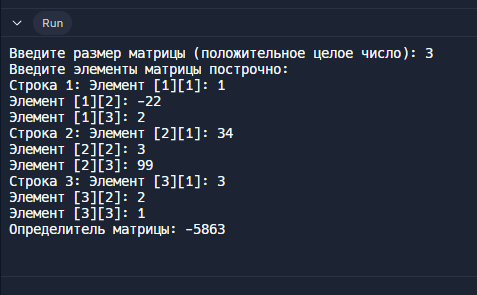
\includegraphics[width=0.5\linewidth]{image.png}
    \caption{Тест программы}
    \label{fig:enter-label}
\end{figure}
\newpage
\section{Список используемой литературы}

\begin{enumerate}
\item Stroustrup, B. The C++ Programming Language. 4th ed. Boston: Addison-Wesley, 2013.

\item Sweeney, D. C++. 2nd ed. New York: McGraw-Hill, 2017.

\item Bjarne Stroustrup. Programming: Principles and Practice Using C++. 2nd ed. Boston: Pearson, 2014.

\item L. P. H. Van de Geijn. Matrix Computations. 3rd ed. Baltimore: Johns Hopkins University Press, 1996.

\item Cormen, T. H., Leiserson, C. E., Rivest, R. L., & Stein, C. Introduction to Algorithms. 3rd ed. Cambridge: MIT Press, 2009.
\end{enumerate}

\end{document}
